\documentclass{article}

\usepackage[utf8]{inputenc}
\usepackage[brazilian]{babel}
\usepackage{graphicx}
\usepackage{float}
\usepackage[pdftex]{hyperref}
\usepackage{epstopdf}
\usepackage{etoolbox}
\usepackage{amsmath}
\usepackage{amsfonts}
\usepackage{amssymb}
\usepackage{caption}
\usepackage{subcaption}
\usepackage{setspace}
\usepackage{tikz}

\patchcmd{\thebibliography}{\section*}{\section}{}{}
\newcommand{\R}{\ensuremath{\mathbb{R}}}
\newcommand{\Prob}{\ensuremath{\mathbb{P}}}
\newcommand{\K}{\ensuremath{\mathbb{K}}}
\newcommand{\U}{\ensuremath{\mathbb{U}}}
\newcommand{\N}{\ensuremath{\mathbb{N}}}
\newcommand{\Lg}{\ensuremath{\mathbb{L}}}
\newcommand{\T}{\ensuremath{\rm Tr}}
\newcommand{\sg}{{\sigma(x_k)}}

\newcommand{\G}{\ensuremath{\mathcal{G}}}
\newcommand{\F}{\ensuremath{\mathcal{F}}}
\newcommand{\C}{\ensuremath{\mathcal{C}}}
\newcommand{\E}{\ensuremath{\mathcal{E}}}
\newcommand{\Hn}{\ensuremath{\mathcal{H}}}
%\newcommand{\Hoo}{\ensuremath{\mathcal{H}_\infty}}
\newcommand{\Hop}{\ensuremath{\mathcal{H}_{op}}}
% --------------------------------------------------
\newtheorem{theo}{Teorema}
\newtheorem{exa}{Exemplo}
\newtheorem{lemm}{Lema}
\newtheorem{coro}{Corolário}
\newtheorem{defn}{Definição}[section]

%opening


\begin{document}
\input{capa.tex}

\onehalfspacing
\section{Objetivos} 
O objetivo desse experimento é realizar a identificação de parâmetros de um motor de corrente contínua com excitação independente de imãs permanentes conforme modelo proposto no roteiro\cite{bb:roteiro}. 
	
\section{Modelo matemático}
O modelo matemático do problema é dividido em duas partes: elétrica e mecânica. A primeira é mostrada na equação \ref{eq:eletrica}, com fonte de tensão V. 

\begin{equation}
\label{eq:eletrica}
BANANA%TODO
\end{equation}
\begin{equation}
\label{eq:mecanica}
BANANA%TODO
\end{equation}
\begin{equation}
\label{eq:gss}
G(s)=BANANA%TODO
\end{equation}
\section{Ensaio com motor parado}
Conforme o roteiro\cite{bb:roteiro}, ao ligar o motor com o eixo travado não geramos força contra-eletromotriz, e com isso conseguimos medir a corrente de armadura $i$ com a adição de um resistor $R_s$ como mostrado na figura \ref{fig:rotparado}. Isso nos possibilita o cálculo dos parâmetros $R [\Omega]$ e $L [H]$ pela equação \ref{eq:rotparado}.

\begin{equation}
\label{eq:rotparado}
i(t) = \frac{V_0}{(R+R_s)}(1-\exp^{-((R+R_s)/L)t})
\end{equation}

\begin{figure}[H]
	\centering
	\includegraphics[width=0.8\linewidth]{rotparado}
	\caption{Circuito para motor com eixo travado}
	\label{fig:rotparado}
\end{figure}

Travando o disco para impossibilitar o motor de girar seu rotor, fizemos o acionamento do módulo de potência, aguardamos a estabilização do sinal de corrente, e desligamento do sistema, obtendo as curvas de corrente e velocidade angular mostradas na figura \ref{fig:ensaiop}.

\begin{figure}[H]
	\centering
	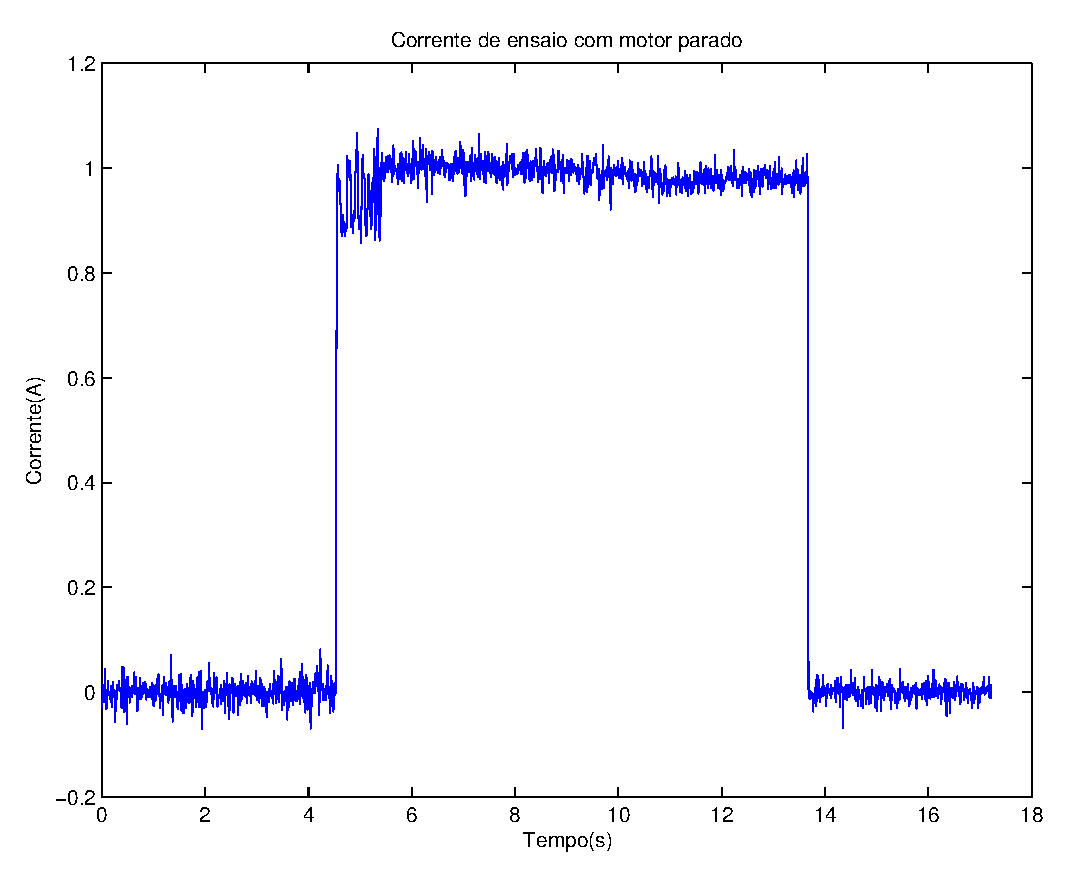
\includegraphics[width=0.8\linewidth]{ensaiop}
	\caption{Corrente e velocidade angular de ensaio com motor parado}
	\label{fig:ensaiop}
\end{figure}

Para o cálculo do parâmetro $R$, utilizamos o valor indicado no roteiro\cite{bb:roteiro} $R_s\approxeq1 \Omega$, a tensão da fonte $V=12 V$ e a partir do momento em que a corrente se estabiliza em $i=%TODO
$, calculamos seu valor conforme \ref{eq:r}.

\begin{equation}
\label{eq:r}
R = \frac{V-R_sI_0}{I_0}=%TODO
\end{equation}

A indutância $L$, por sua vez, é calculada utilizando a constante de tempo da parte elétrica onde a corrente passa a ser $63\%$ do valor de regime, $i(\tau_e)=(1-\exp^{-1})I_0$ e portanto
$\tau_e=%TODO
$, de acordo com a equação \ref{eq:l}.

\begin{equation}
\label{eq:l}
L = \tau_e(R+R_s)=%TODO
\end{equation}

\section{Ensaio com motor em movimento}

\section{Resultados finais}
Com todos os parâmetros necessários calculados, substituindo os valores em \ref{eq:gss}, obtemos a planta dada pela equação \ref{eq:gs}.

\begin{equation}
\label{eq:gs}
G(s)=%TODO
\end{equation}

%TODO: ANÁLISES ANÁLISES ANÁLISES ANANÁS BANANAS

\begin{thebibliography}{widestlabel}
	\bibitem{bb:roteiro}{Roteiro do experimento disponibilizado para os alunos}
\end{thebibliography}
\end{document}

